%!TEX root = ../report.tex
\chapter{Methodology}

\section{Experimental Design}
\label{sec:experimental_design}
A planar mobile robot with a kinematic model is spawned at initial position. 
The robot needs to travel to the goal position and it should avoid collision with static and moving obstacles. 
A collision is considered to happen when the physical body (model in case of simulation)
is in contact with physical body of the obstacle.
The position of the robot in the environment is available to the motion planner.
A global planner is also available to the motion planner if it needs one.
The position, velocity and shape of the moving obstacle is also available to the motion
planner.
The experiment is performed multiple times and each time following things are measured
\begin{itemize}
    \item time to reach goal
    \item number of collisions
    \item number of times motion planner had to re-plan
\end{itemize}
All these values are expected to be minimum for a better planner.

Re-plan attempts signify how well a planner considers the information it receives. According to
the safety criteria in~\cite{fraichard2007short}, a planner should take into account the future behaviour
of its environment and make decision accordingly. This implies that an ideal planner will only have
to plan once. The equivalent of this in real scenario is that a planner will update its plan at 
regular interval but it is never forced to completely re-plan because the previous plan was no longer 
viable. Thus, lower re-plan count is more desirable. 

Travel time also needs to be as low as possible. All the planners are configured to minimise time.
Another possibility is to minimise the travel distance. The difference in behaviour will be that 
when the robot encounters a moving obstacle that is blocking its path, the planner will try to pass
the obstacles rather than wait for obstacles to clear its way. For indoor applications, the planner
does not need to worry about the distance. However, for outdoor applications, minimising travel
distance might be desirable.

\section{Setup}
\label{sec:setup}

A gazebo simulator\cite{koenig2004design} is used for simulating the desired environment on a laptop
machine (Refer~\ref{sec:machine_specifications} for machine specifications).
KUKA youbot\cite{bischoff2011kuka} is used as the robot model. The robot is operated using ROS\cite{quigley2009ros}. It is an
omni-directional robot which is steered as holonomic vehicle for the experiments 
(Refer~\ref{sec:kinodynamic_parameters} for parameters). It is equipped with 2 laser range finders
which are placed in the front and back of the robot. The laser range finder have a field of view of
190$^o$. These can be used to localise the robot or update costmap\cite{costmap}. However, they create
a blind spot in the robot's field of view (on either side of the robot).

Global planner\cite{globalPlanner} is used from ROS navigation\cite{rosnavigation} if required. 
A planner is free to use AMCL\cite{amcl} or truth value directly from simulator to get the
robot's current position. If the planner uses AMCL, we localise the robot before starting
motion planning.

Travel time is measured from the moment goal position is given to motion planner to the 
time when robot reached goal position and stops moving (For goal tolerance parameters refer~\ref{sec:goal_tolerance_parameters}).
The number of re-plan attempts are measured by manually counting each instance when the motion
planner has to re-plan but the global planner did not re-plan.
Number of collisions were measured by manually counting the number of times robot collided with any
obstacle (static or moving) in simulator.

We run the planner multiple times to be unbiased against the position of moving obstacle 
at start time.
Additionally, we also run the planner in static environment to obtain a benchmark.
All obstacles are cylinders of diameter 30 cm and height 50 cm. None of the obstacles move 
faster than 0.4 m/s. All obstacles follow a `to and fro' motion. The obstacles have 
linear acceleration and deceleration. This implies that their velocity is constantly changing as shown
in Figure~\ref{fig:moving_obs_velocity_plots}.

\section{Test case 1: Single obstacle single room}%
\label{sec:test_case_1_single_obstacle_single_room}
    This test case is similar to the classic road crossing benchmark\cite{van2008reciprocal}. The goal 
    is in line of sight of the robot. The motion planner does not need to rely on 
    global planner. A single obstacle is moving between the robot and the goal as shown in 
    Figure~\ref{fig:single_obs_single_room}. The velocity of the moving obstacle is constantly changing as shown in 
    Figure~\ref{fig:single_obs_velocity_plot}. The size of the room is 4 meters in length and 3 
    meters in width. This represents a small room or a small subsection of a large room in a 
    typical indoor environment. Apart from walls of the room, no additional static obstacles are
    simulated. The robot starts at \texttt{x=-1.0, y=0.0, theta=0.0} and the goal is at \texttt{x=1.0, y=1.0, theta=0.0}.
    The maximum opening for the robot is 2.7 meters when the obstacles is at the 
    end points of its linear path. 
\begin{figure}[ht]
    \centering
    \begin{subfigure}[b]{0.50\linewidth}
        \centering
        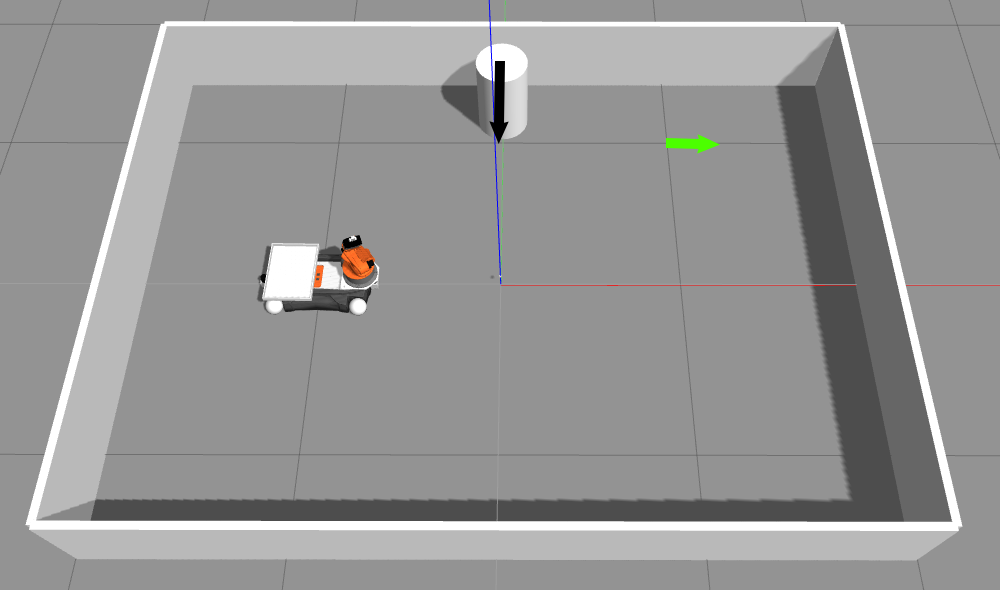
\includegraphics[width=0.95\textwidth]{images/test_case_1/exp1.png}
        \caption{t=0.0s}
    \end{subfigure}%
    \begin{subfigure}[b]{0.50\linewidth}
        \centering
        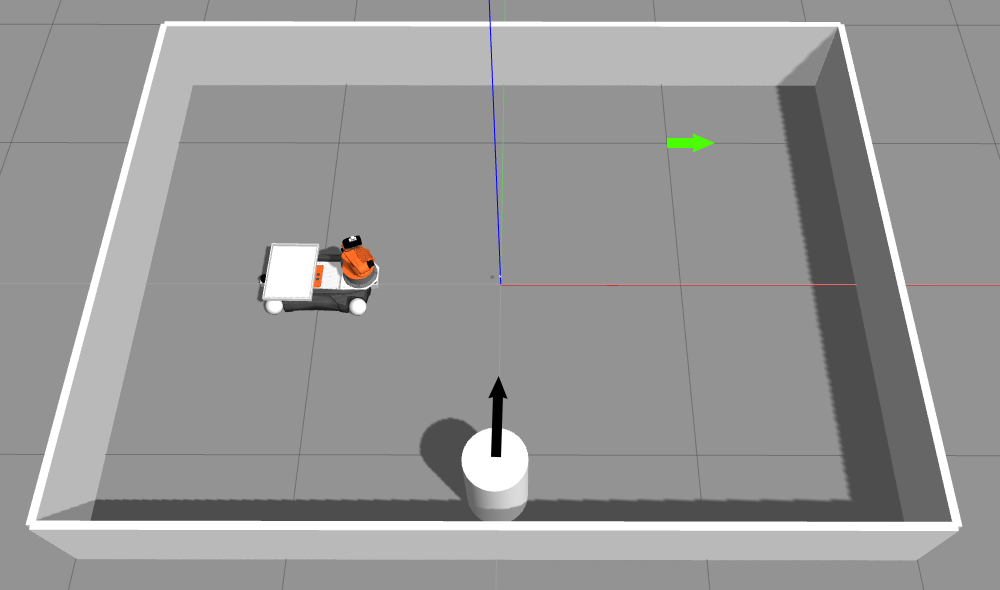
\includegraphics[width=0.95\textwidth]{images/test_case_1/exp3.png}
        \caption{t=10.0s}
    \end{subfigure}%
    \caption{Test case 1 obstacle trajectory (green arrow is goal position)}\label{fig:single_obs_single_room}
\end{figure}

\section{Test case 2: Two obstacle single room}%
\label{sec:test_case_2_two_obstacle_single_room}
    The goal is still in line of sight of the robot. This test case is a logical extension of
    the previous test case. There are 2 obstacles between the robot and the goal. The difficulty
    is almost double because the opening for the robot is always less than 1.7 meters. This is 
    because the obstacles are offset by 50\% of their journey as shown in Figure~\ref{fig:two_obstacle_single_room}.
    The initial and goal positions are same as test case 1. The second obstacle (the obstacle moving 
    diagonally) slows down near origin to coordinate with the offset. This can be seen in Figure~\ref{fig:second_obs_velocity_plot}.
\begin{figure}[H]
    \centering
    \begin{subfigure}[b]{0.50\linewidth}
        \centering
        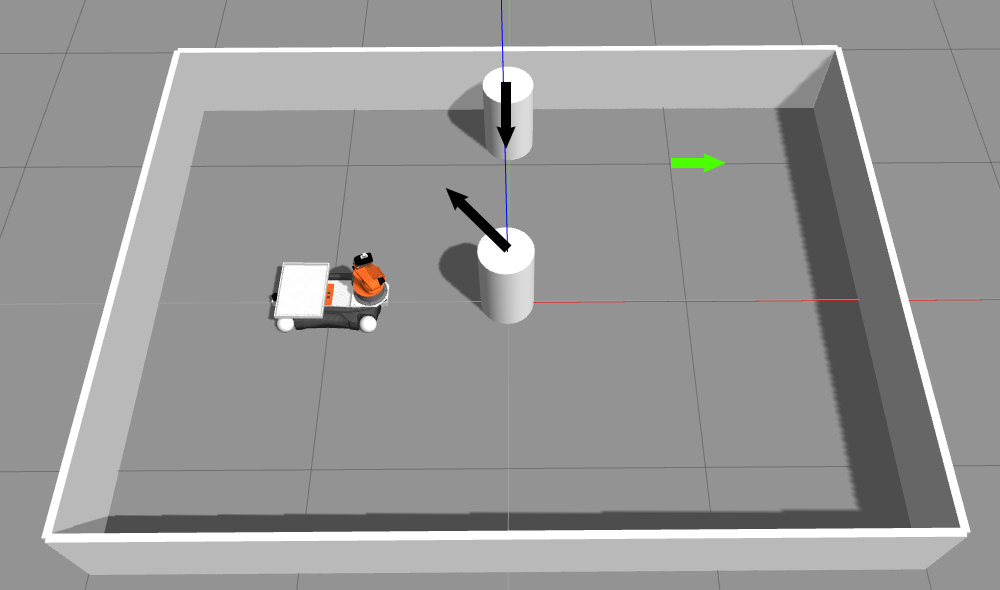
\includegraphics[width=0.95\textwidth]{images/test_case_2/exp1.png}
        \caption{t=0.0s}
    \end{subfigure}%
    \begin{subfigure}[b]{0.50\linewidth}
        \centering
        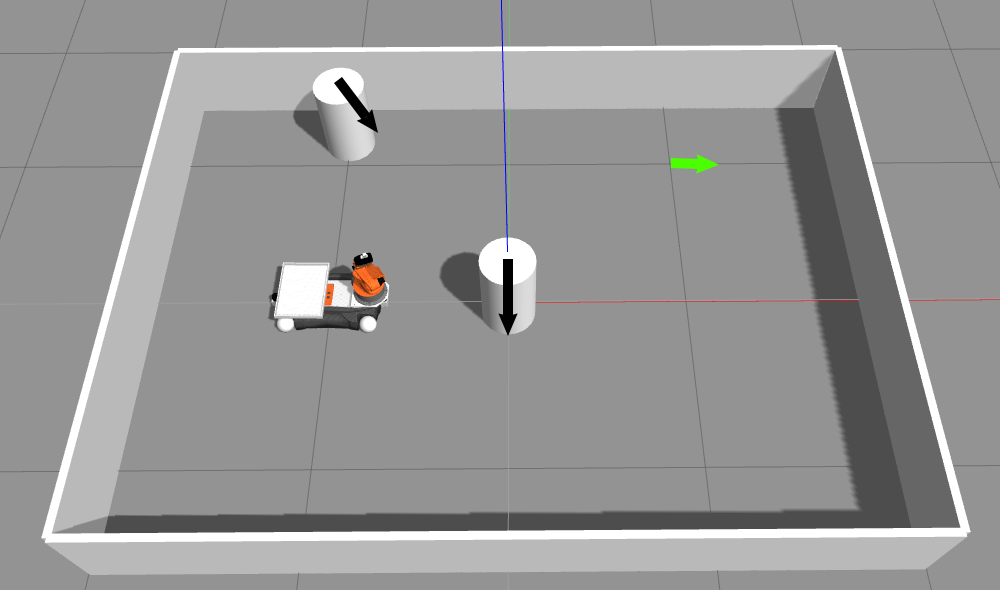
\includegraphics[width=0.95\textwidth]{images/test_case_2/exp2.png}
        \caption{t=5.0s}
    \end{subfigure}
    \begin{subfigure}[b]{0.50\linewidth}
        \centering
        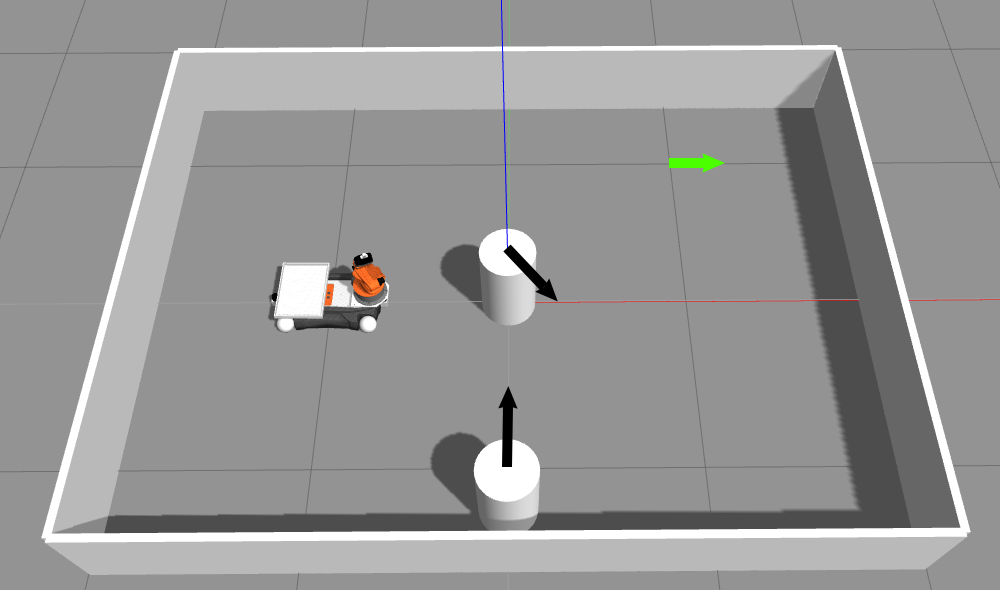
\includegraphics[width=0.95\textwidth]{images/test_case_2/exp3.png}
        \caption{t=10.0s}
    \end{subfigure}%
    \begin{subfigure}[b]{0.50\linewidth}
        \centering
        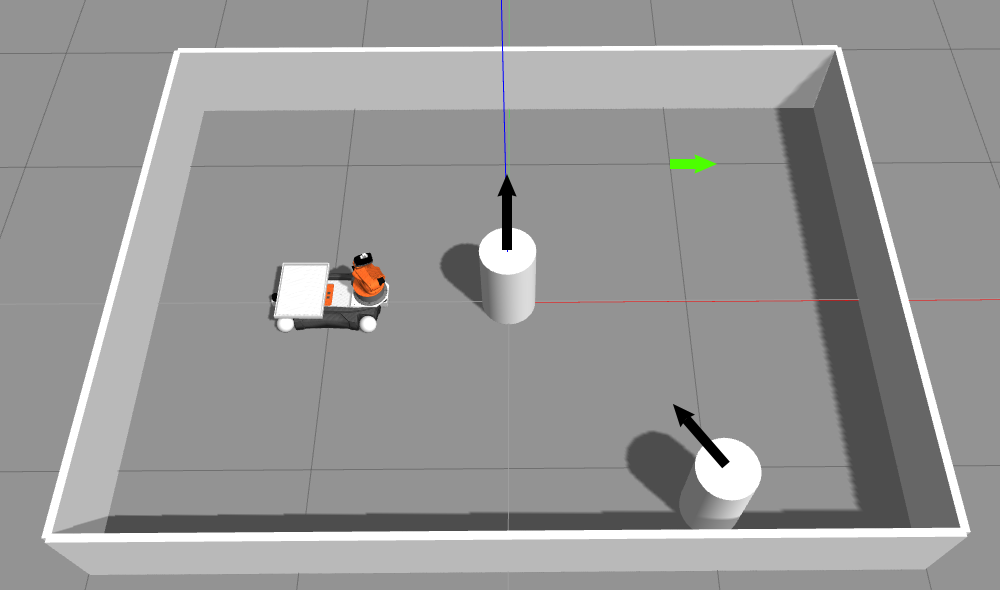
\includegraphics[width=0.95\textwidth]{images/test_case_2/exp4.png}
        \caption{t=15.0s}
    \end{subfigure}%
    \caption{Test case 2 obstacle trajectories (green arrow is goal position)}\label{fig:two_obstacle_single_room}
\end{figure}

\section{Test case 3: Double room}%
\label{sec:test_case_3_double_room}
    Unlike the previous test cases, the goal is not in line of sight in this test case. The 
    robot has to exit its current room, travel through a corridor filled with moving obstacles 
    and enter another room to get to the goal position. The corridor is 2 meters wide and 8 meters
    in length. 

    The corridor contains 6 obstacles which move in 3 parallel tracks as shown in Figure~\ref{fig:double_room}.
    We expect a zigzag trajectory from an ideal motion planner. However, the ideal planner still 
    would have to wait for the obstacles to move near time \texttt{t=0.0s} and \texttt{t=15.0s} and 
    their multiples.
    Additionally, there is one obstacle in the room the robot is spawned and 2 moving obstacles in 
    the next room. All obstacles have the same velocity for their trajectory, only their directions
    are different. The velocity of the moving obstacles in this test case 
    (Figure~\ref{fig:third_obs_velocity_plot}) is almost same as test case 1,
    the only difference is the time of their travel is extended before they repeat their behaviour. 
    This makes their maximum velocity a little less than the maximum velocity of moving obstacles in 
    test case 1.
    The robot starts at \texttt{x=-1.0, y=0.0, theta=0.0} and the goal position is \texttt{x=3.0, y=-1.0, theta=0.0}.

\begin{figure}[H]
    \centering
    \begin{subfigure}[b]{0.50\linewidth}
        \centering
        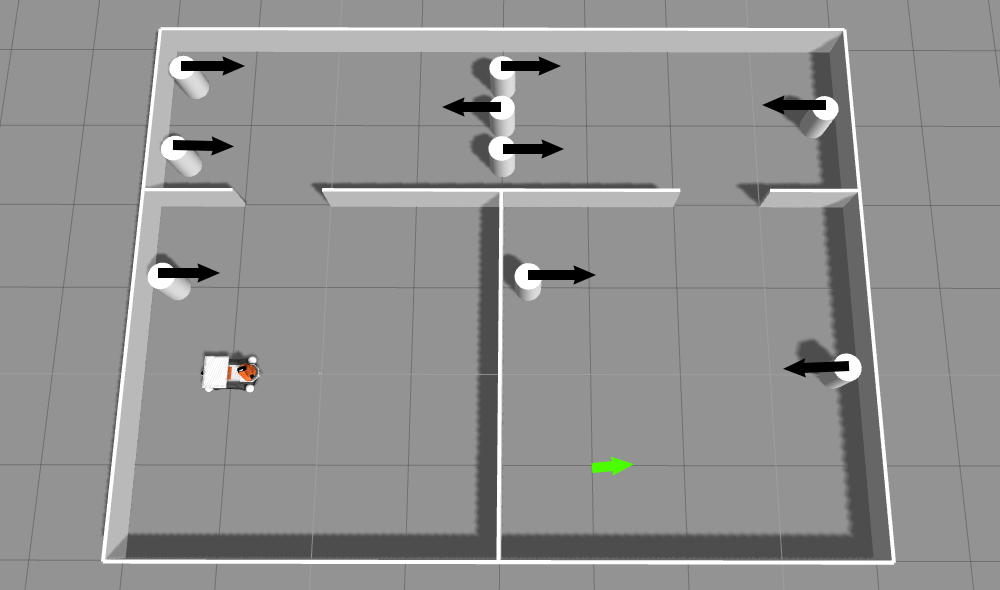
\includegraphics[width=0.95\textwidth]{images/test_case_3/exp1.png}
        \caption{t=0.0s}
    \end{subfigure}%
    \begin{subfigure}[b]{0.50\linewidth}
        \centering
        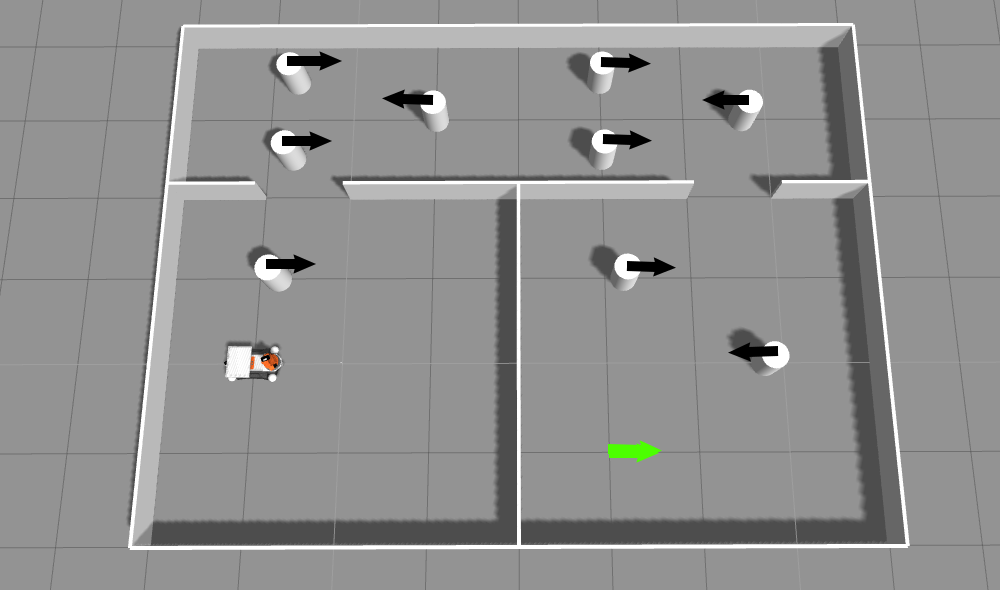
\includegraphics[width=0.95\textwidth]{images/test_case_3/mid1.png}
        \caption{t=5.0s}
    \end{subfigure}
    \begin{subfigure}[b]{0.50\linewidth}
        \centering
        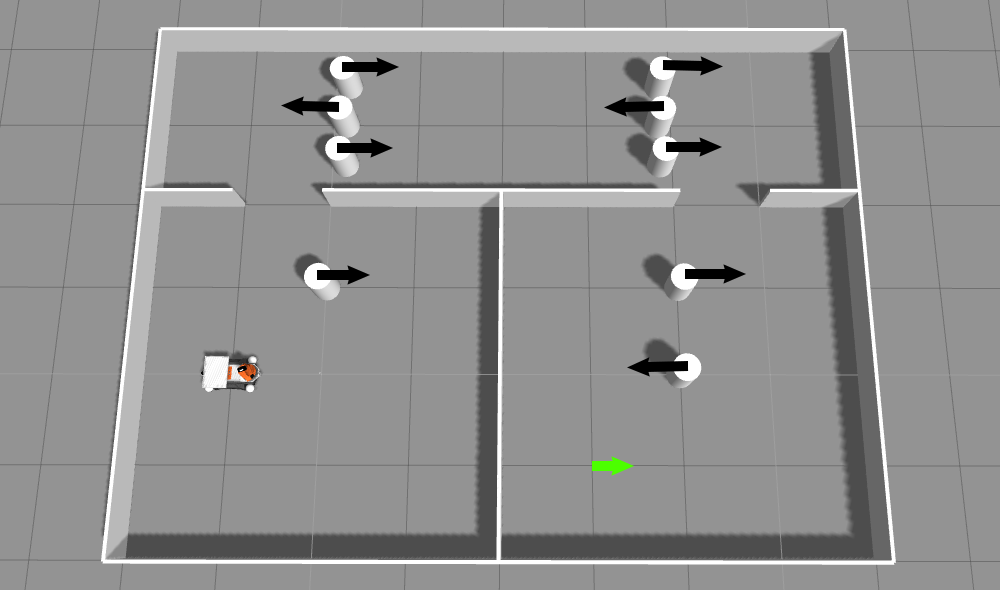
\includegraphics[width=0.95\textwidth]{images/test_case_3/exp2.png}
        \caption{t=7.5s}
    \end{subfigure}%
    \begin{subfigure}[b]{0.50\linewidth}
        \centering
        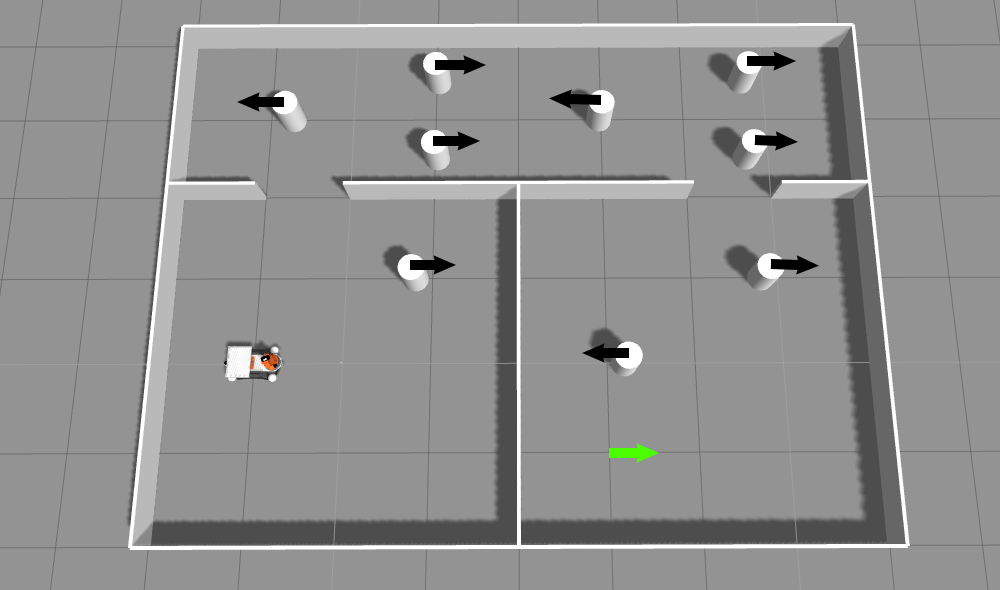
\includegraphics[width=0.95\textwidth]{images/test_case_3/mid2.png}
        \caption{t=10.0s}
    \end{subfigure}
    \begin{subfigure}[b]{0.50\linewidth}
        \centering
        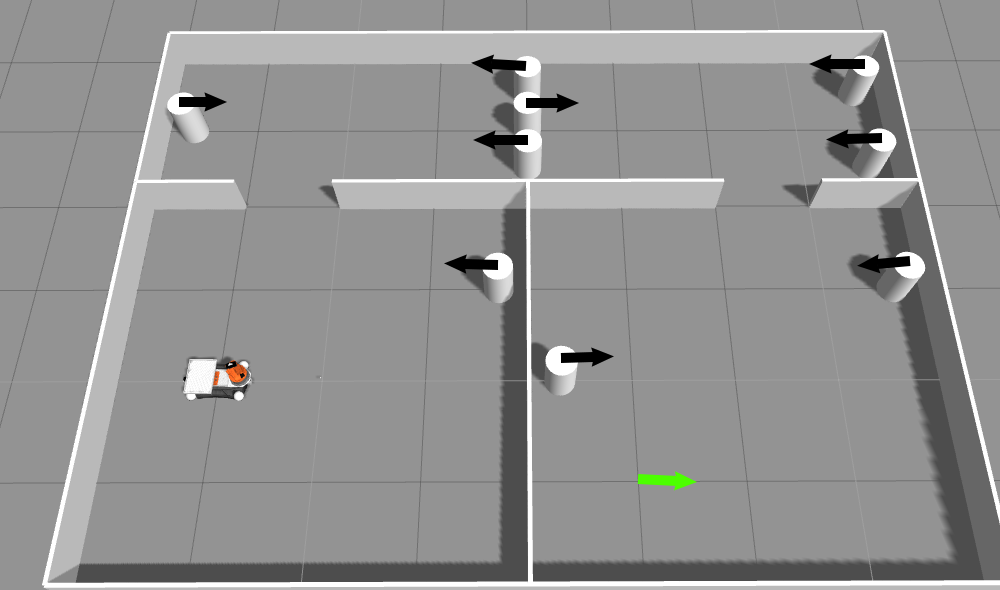
\includegraphics[width=0.95\textwidth]{images/test_case_3/exp3.png}
        \caption{t=15.0s}
    \end{subfigure}%
    \begin{subfigure}[b]{0.50\linewidth}
        \centering
        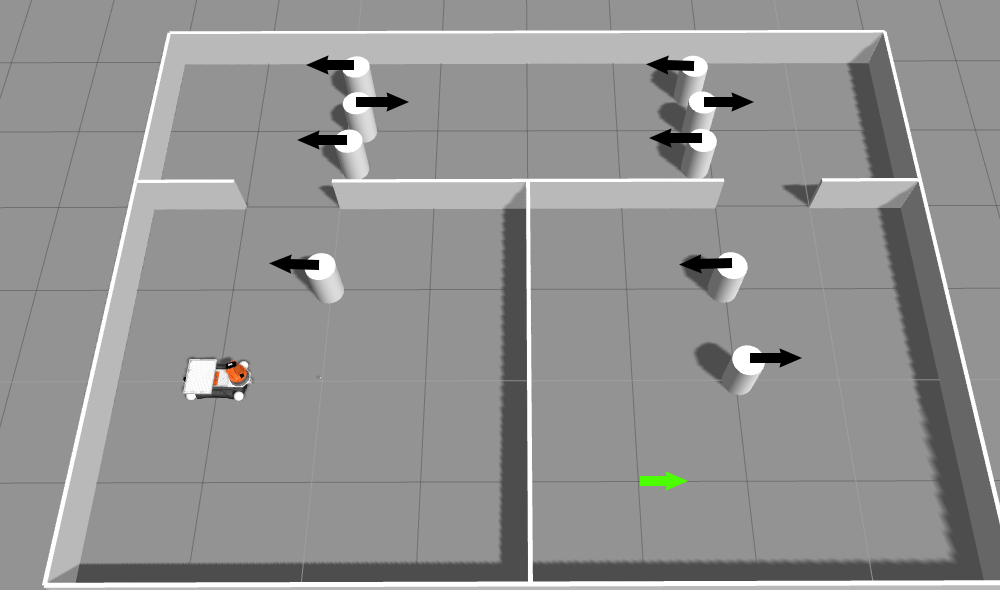
\includegraphics[width=0.95\textwidth]{images/test_case_3/exp4.png}
        \caption{t=22.5s}
    \end{subfigure}
    \caption{Test case 3 velocity trajectories (green arrow is goal position)}\label{fig:double_room}
\end{figure}

\begin{figure}[H]
    \centering
    \begin{subfigure}[b]{0.70\linewidth}
    \centering
    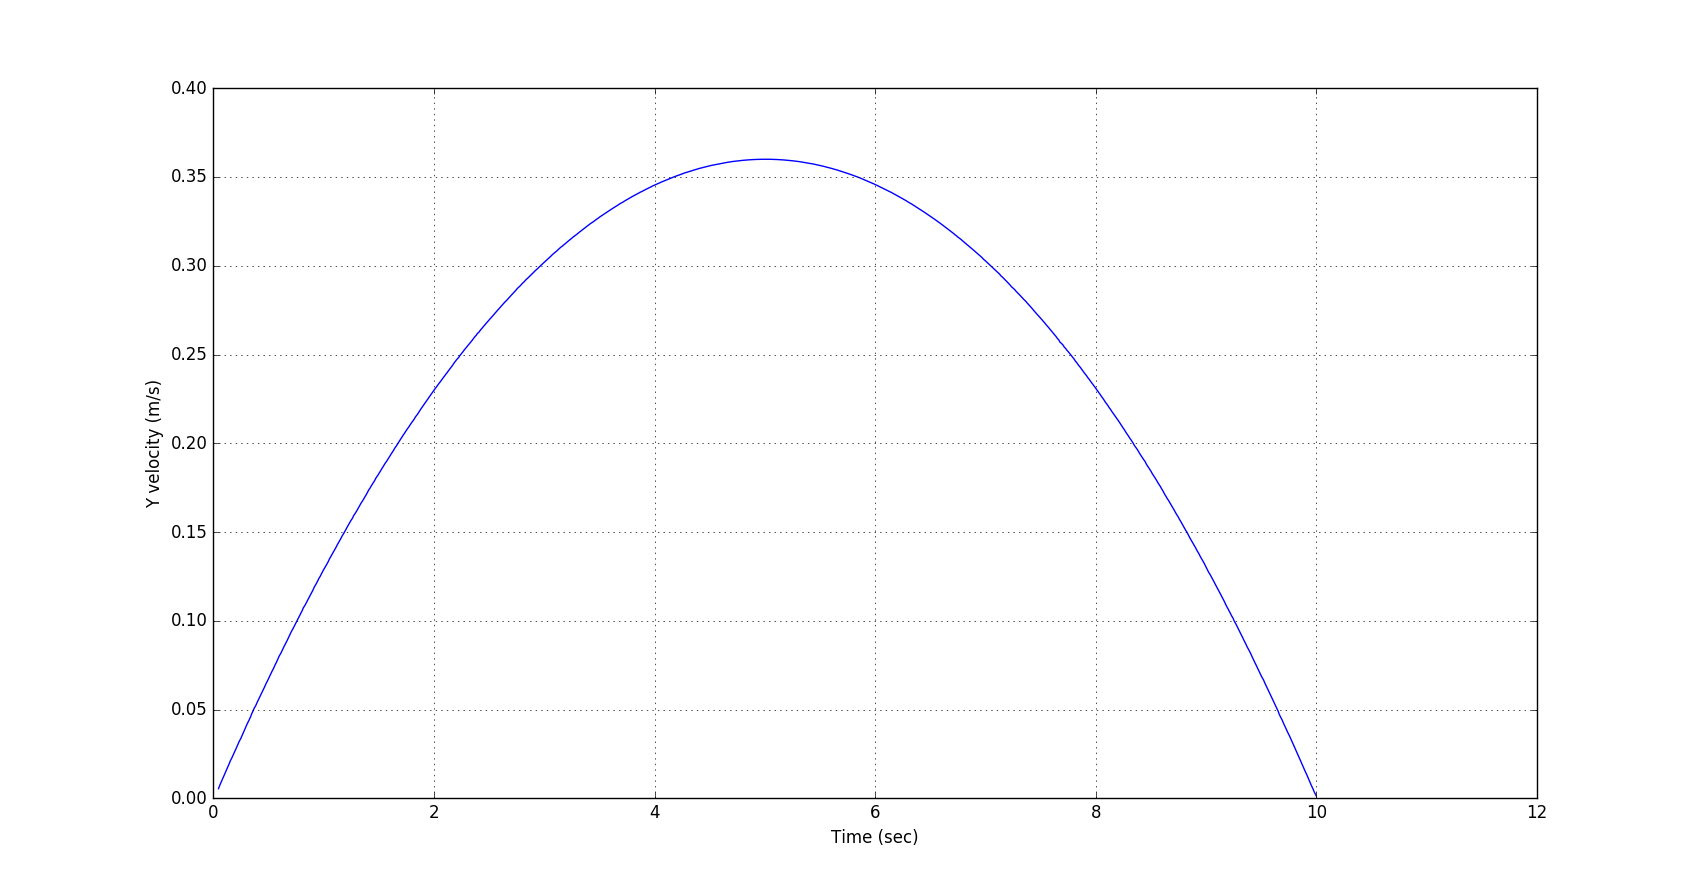
\includegraphics[width=0.8\linewidth]{images/velocity_obs_0.png}
    \caption{\label{fig:single_obs_velocity_plot} First obstacle in test case 1 and 2 (the obstacle moving vertically)}
    \end{subfigure}
    \begin{subfigure}[b]{0.70\linewidth}
    \centering
    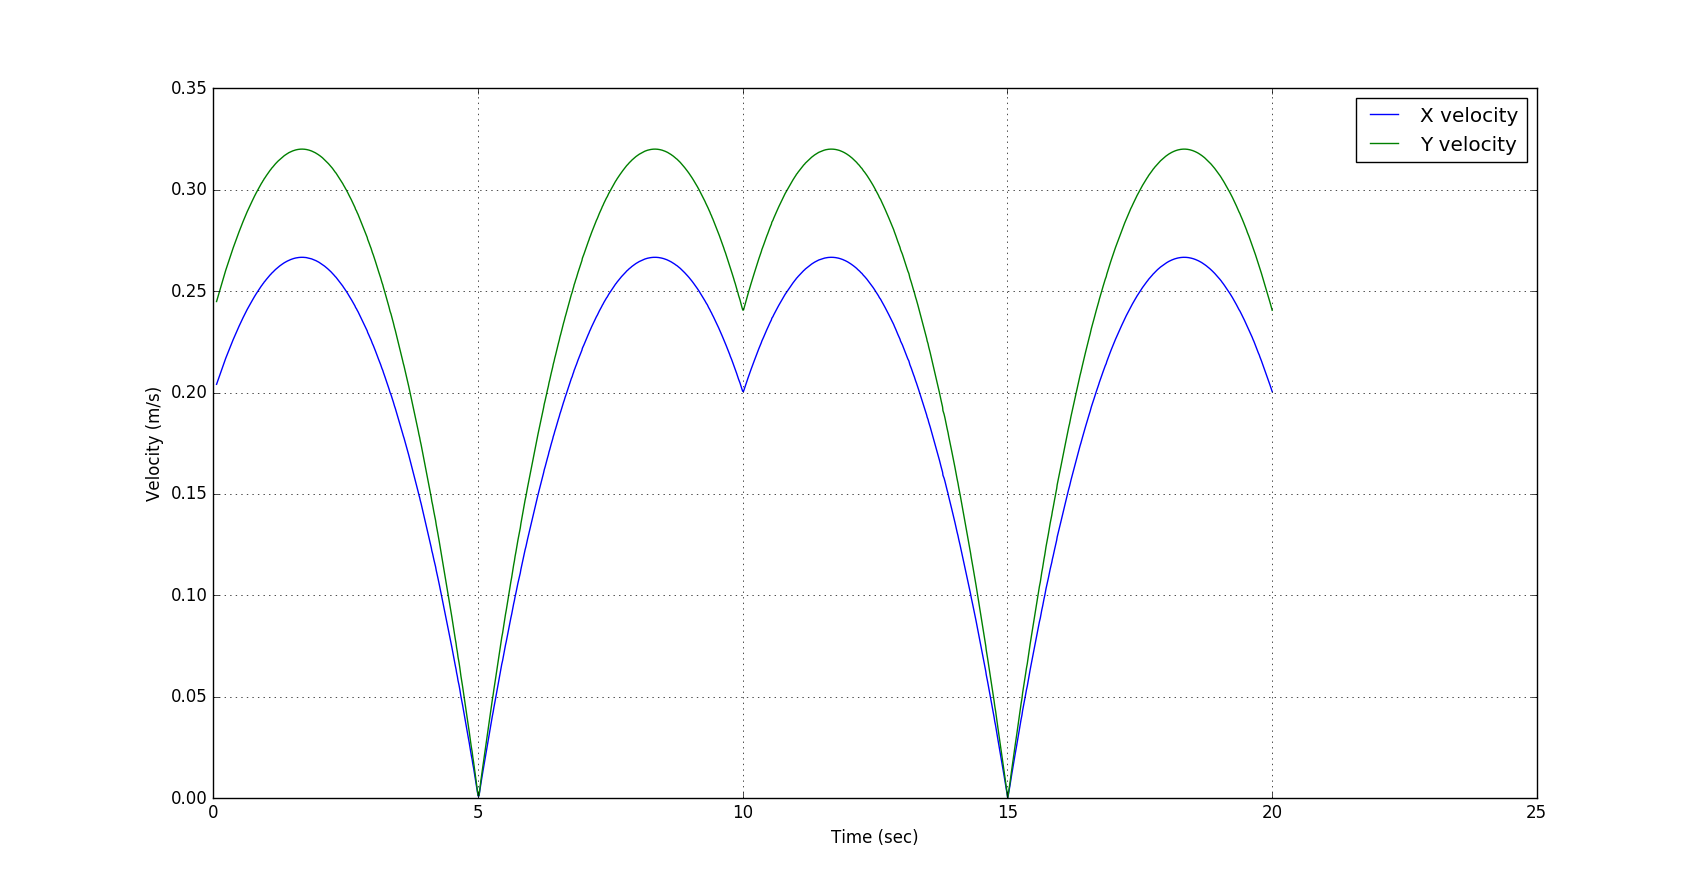
\includegraphics[width=0.8\linewidth]{images/velocity_obs_1.png}
    \caption{\label{fig:second_obs_velocity_plot} Second obstacle in test case 2 (the obstacle moving diagonally)}
    \end{subfigure}
    \begin{subfigure}[b]{0.70\linewidth}
        \centering
        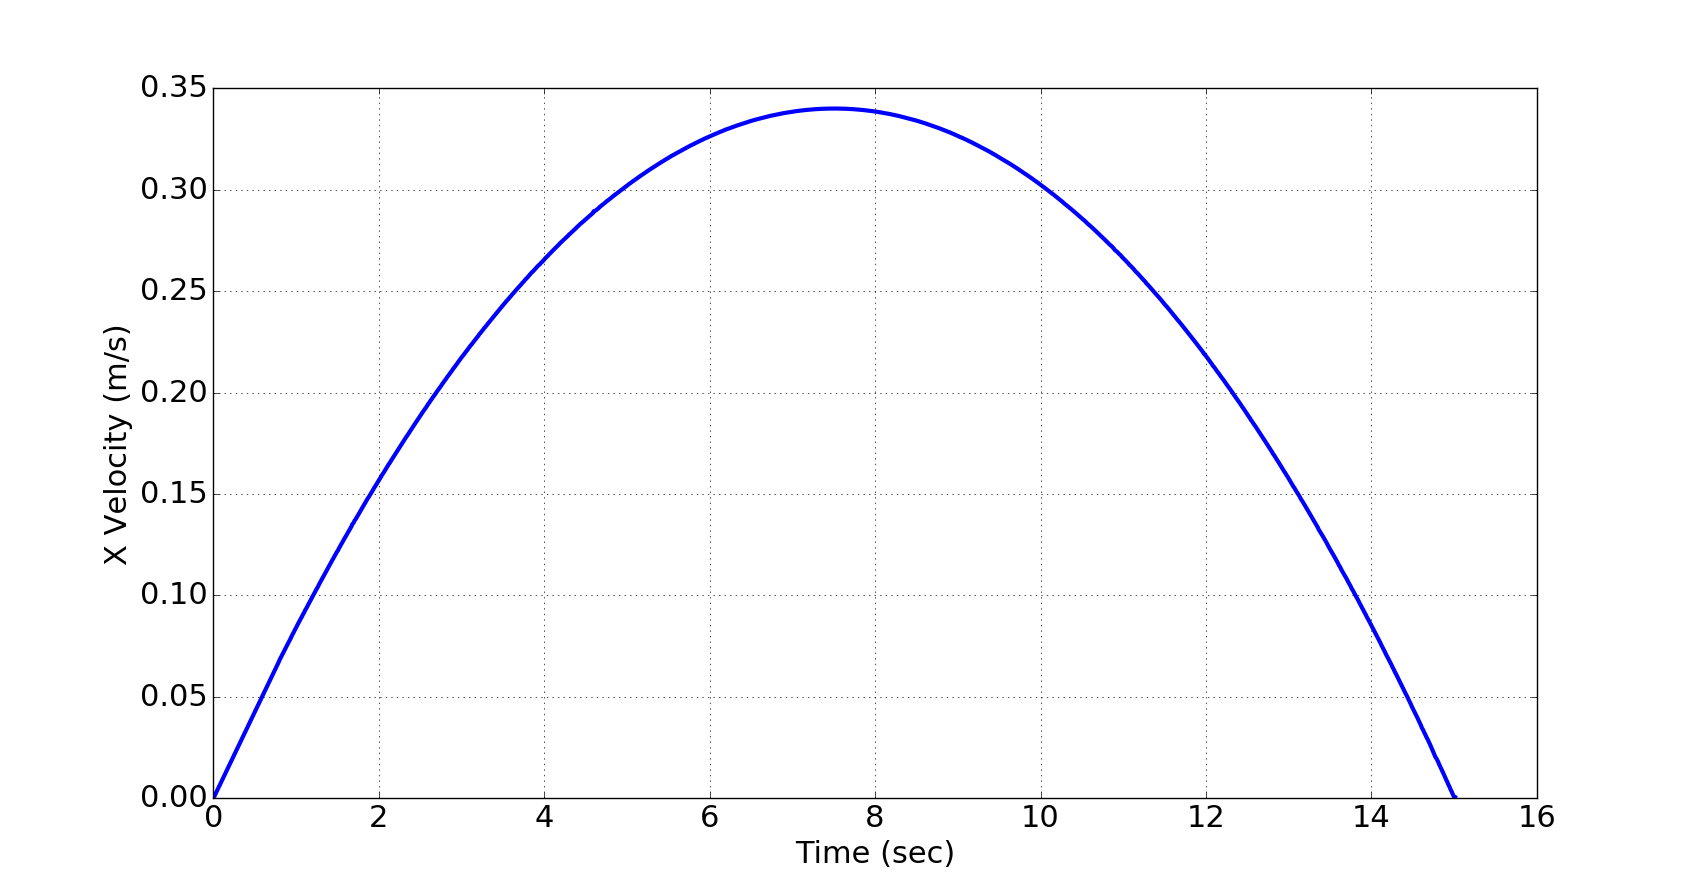
\includegraphics[width=0.95\linewidth]{images/velocity_obs_2.png}
        \caption{\label{fig:third_obs_velocity_plot} Obstacles in test case 3}
    \end{subfigure}
    \caption{\label{fig:moving_obs_velocity_plots} Velocity vs.\ time plot for moving obstacles}
\end{figure}

